\chapter{Rapporten}

\section{Recente logs} \index{logs}
    Gebeurtenissen bekijken die recent zijn gelogd.
De DBlog-module \index{dblog-module} bewaakt de website en slaat
systeemgebeurtenissen op in een logboek dat iedere gebruiker met toestemming op een later tijdstip kan bekijken. 
Het logboek \index{logboek} is een eenvoudige lijst van geregistreerde
gebeurtenissen zoals gebruiks- en prestatiegegevens, fouten, waarschuwingen en operationele informatie. 
Aangezien het logboek vaak de enige bron van informatie is, is het belangrijk dat dit 
regelmatig gecontroleerd wordt.
 \begin{figure}[!h]
    \centering
   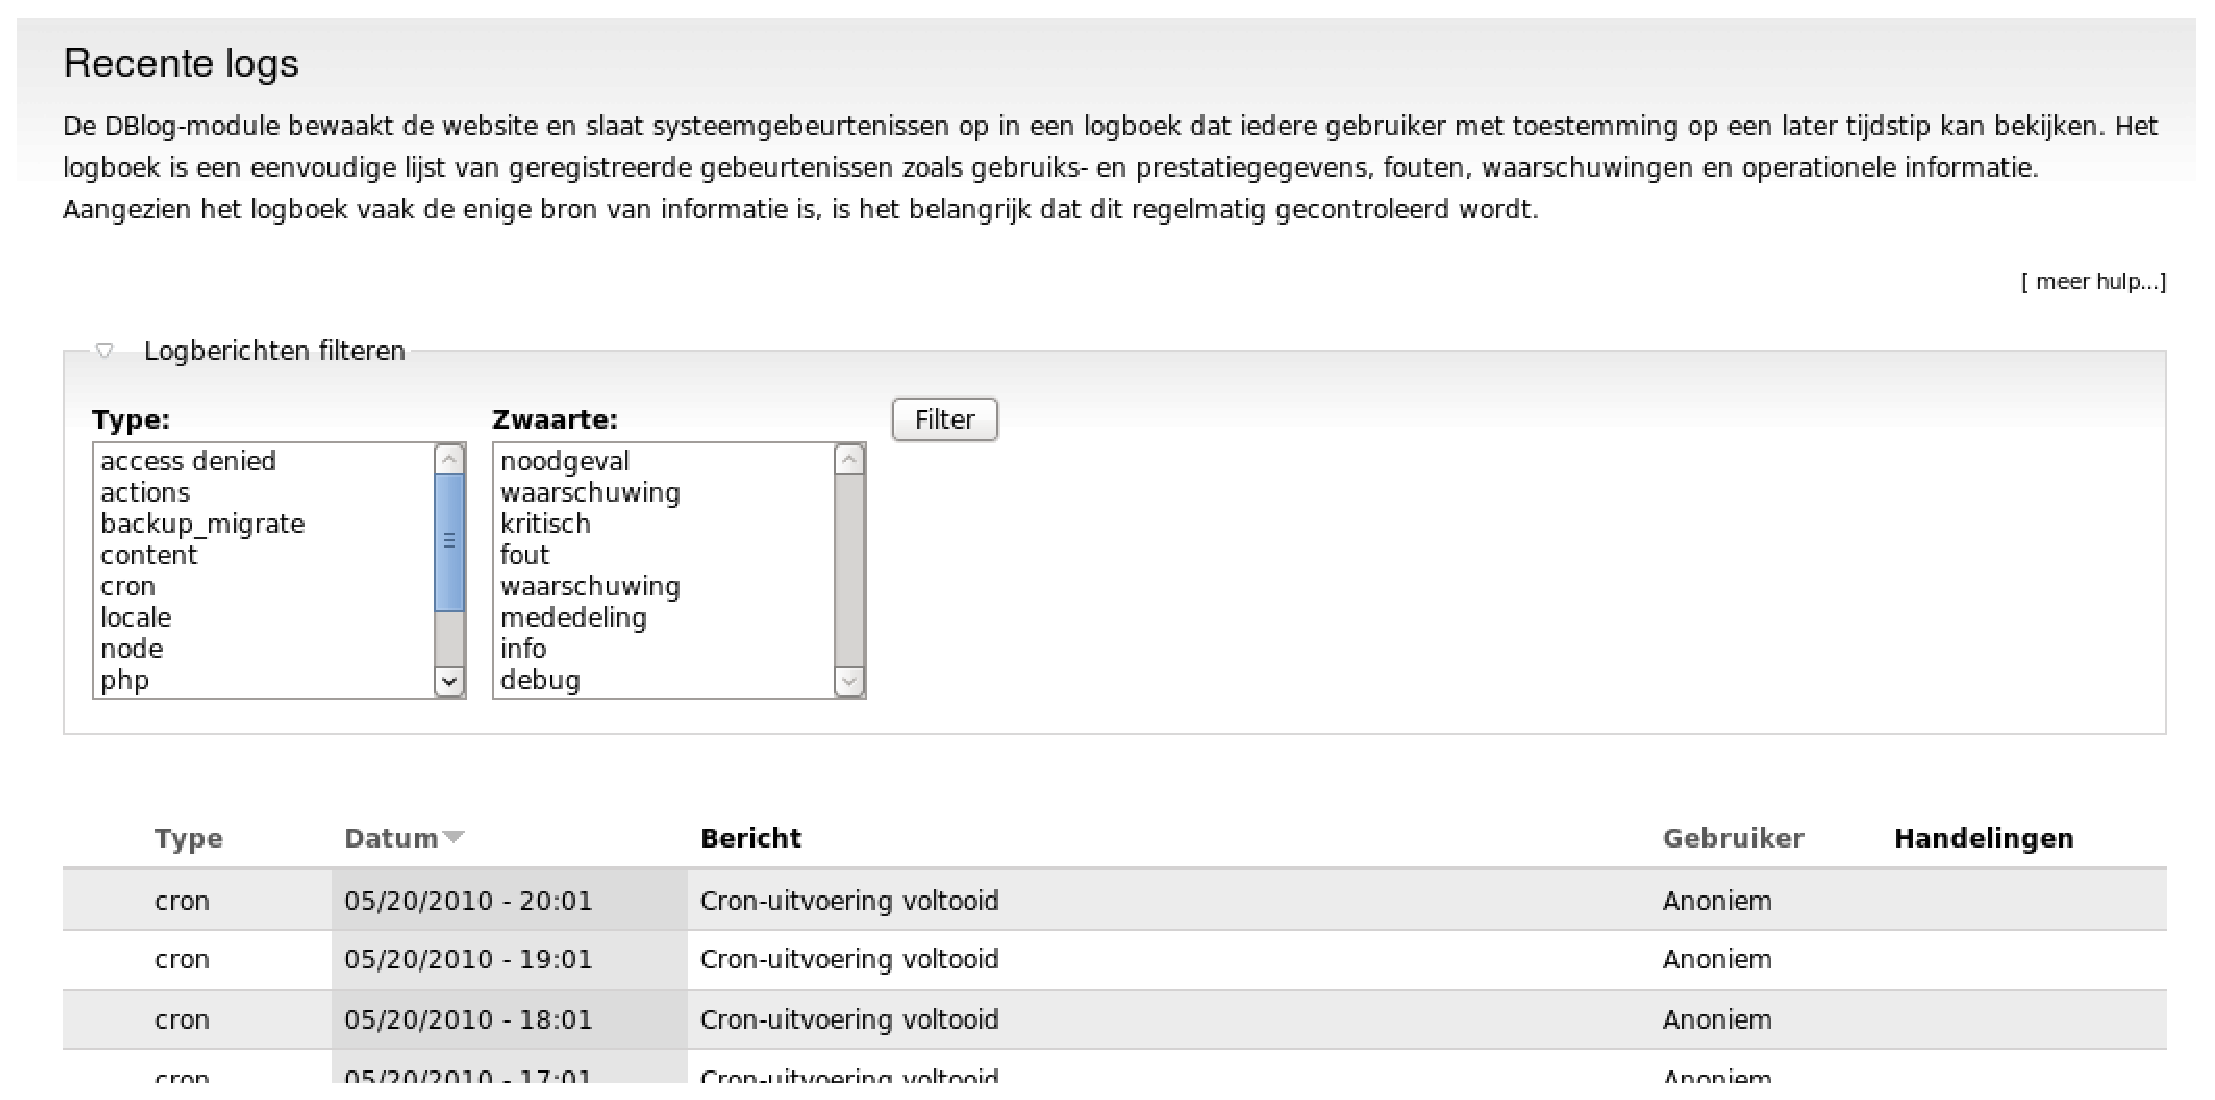
\includegraphics[scale=0.4,angle=0]{recente-logs1}
   \caption{recente-logs1.\label{white}}
 %  \small \\Drupal
 \end{figure}
    
\subsection{Database logging}
De DBlog-module bewaakt de website en slaat systeemgebeurtenissen op in een logboek dat iedere gebruiker
 met toestemming op een later tijdstip kan bekijken. Dit is nuttig voor sitebeheerders die een snel overzicht
willen van activiteiten op de site. Het logboek slaat ook de volgorde van de gebeurtenissen op, 
wat nuttig kan zijn om fouten op de site op te lossen.
\\
Het dblog-logboek is een eenvoudige lijst van geregistreerde gebeurtenissen zoals gebruiks- en prestatiegegevens, 
fouten, waarschuwingen en operationele informatie. Beheerders zouden regelmatig de dblog moeten controleren om er 
zeker van te zijn dat de site goed functioneert.
\\\\
opm: Lees voor meer informatie het online-handboek over de Dblog-module.
 \begin{figure}[!h]
    \centering
   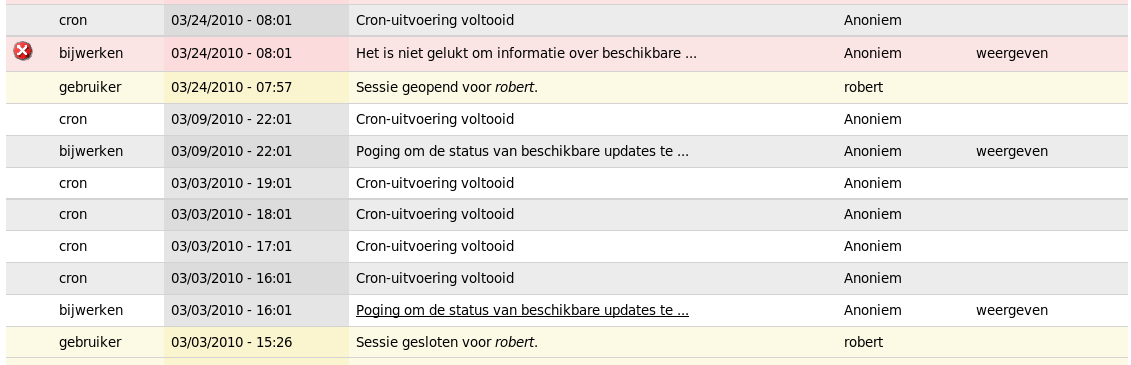
\includegraphics[scale=0.4,angle=0]{recente-logs2}
   \caption{recente-logs2.\label{white}}
 %  \small \\Drupal
 \end{figure}
\subsection{Database logging beheerpagina's}
\begin{itemize}
 \item Database loggen
 \item Meest voorkomende fouten 'Geen toegang'
 \item Meest voorkomende fouten 'pagina niet gevonden'
 \item Recente logs
\end{itemize}

\section{Meest populaire zoekwoorden} \index{zoekwoorden}
    Bekijk de meest populaire zoekwoorden
\begin{figure}[!h]
    \centering
   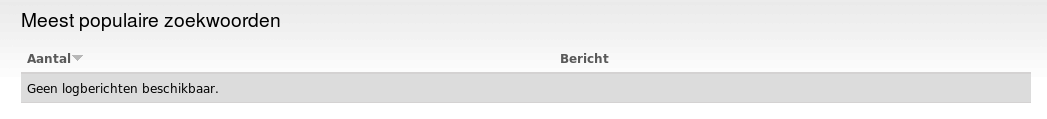
\includegraphics[scale=0.4,angle=0]{populaire-zoekwoorden}
   \caption{populaire-zoekwoorden.\label{white}}
 %  \small \\Drupal
 \end{figure}    
    
    
\section{Meest voorkomende fouten 'Geen toegang'\index{fout - geen toegang}} 
    'Geen toegang' fouten (403) bekijken.
\begin{figure}[!h]
    \centering
   
\includegraphics[scale=0.4,angle=0]{geen-toegang}
   \caption{geen-toegang.\label{white}}
 %  \small \\Drupal
 \end{figure}     
    
    
\section{Meest voorkomende fouten 'pagina niet gevonden'\index{fout - niet
gevonden}}  'Pagina niet gevonden' fouten (404) bekijken.
\begin{figure}[!h]
    \centering
   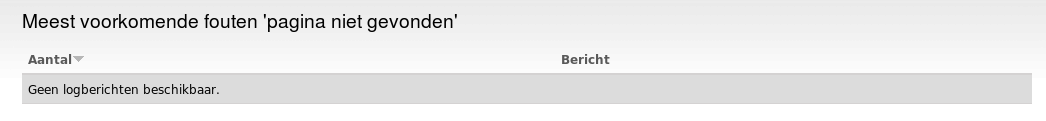
\includegraphics[scale=0.4,angle=0]{pagina-niet-gevonden}
   \caption{pagina-niet-gevonden.\label{white}}
 %  \small \\Drupal
 \end{figure} 



\section{Beschikbare updates} \index{updates}
    Ontvang een statusrapport van beschikbare nieuwe versies voor
 ge\"installeerde modules en templates.
\\
Hier vindt u meer informatie over beschikbare nieuwe versies voor de
ge\"installeerde modules en templates. Let op, iedere module of template is een
onderdeel van een 'project' dat dezelfde of een andere naam kan hebben en meerdere modules of templates kan omvatten.\\
Een groot aantal uitbreidingsmodules en uitbreidingstemplates zijn beschikbaar om de functionaliteit van 
uw website uit te breiden of de layout te wijzingen.\\
Laatste controle: 1 sec geleden (Handmatig controleren)\\
Er is geen informatie beschikbaar over potenti\"ele updates voor de
ge\"installeerde modules en templates. Om op nieuwe versies te controleren
kunt u cron instellen of kunt u handmatig controleren. Even geduld, het controleren op nieuwe versies kan enige tijd duren.
\begin{figure}[!h]
    \centering
   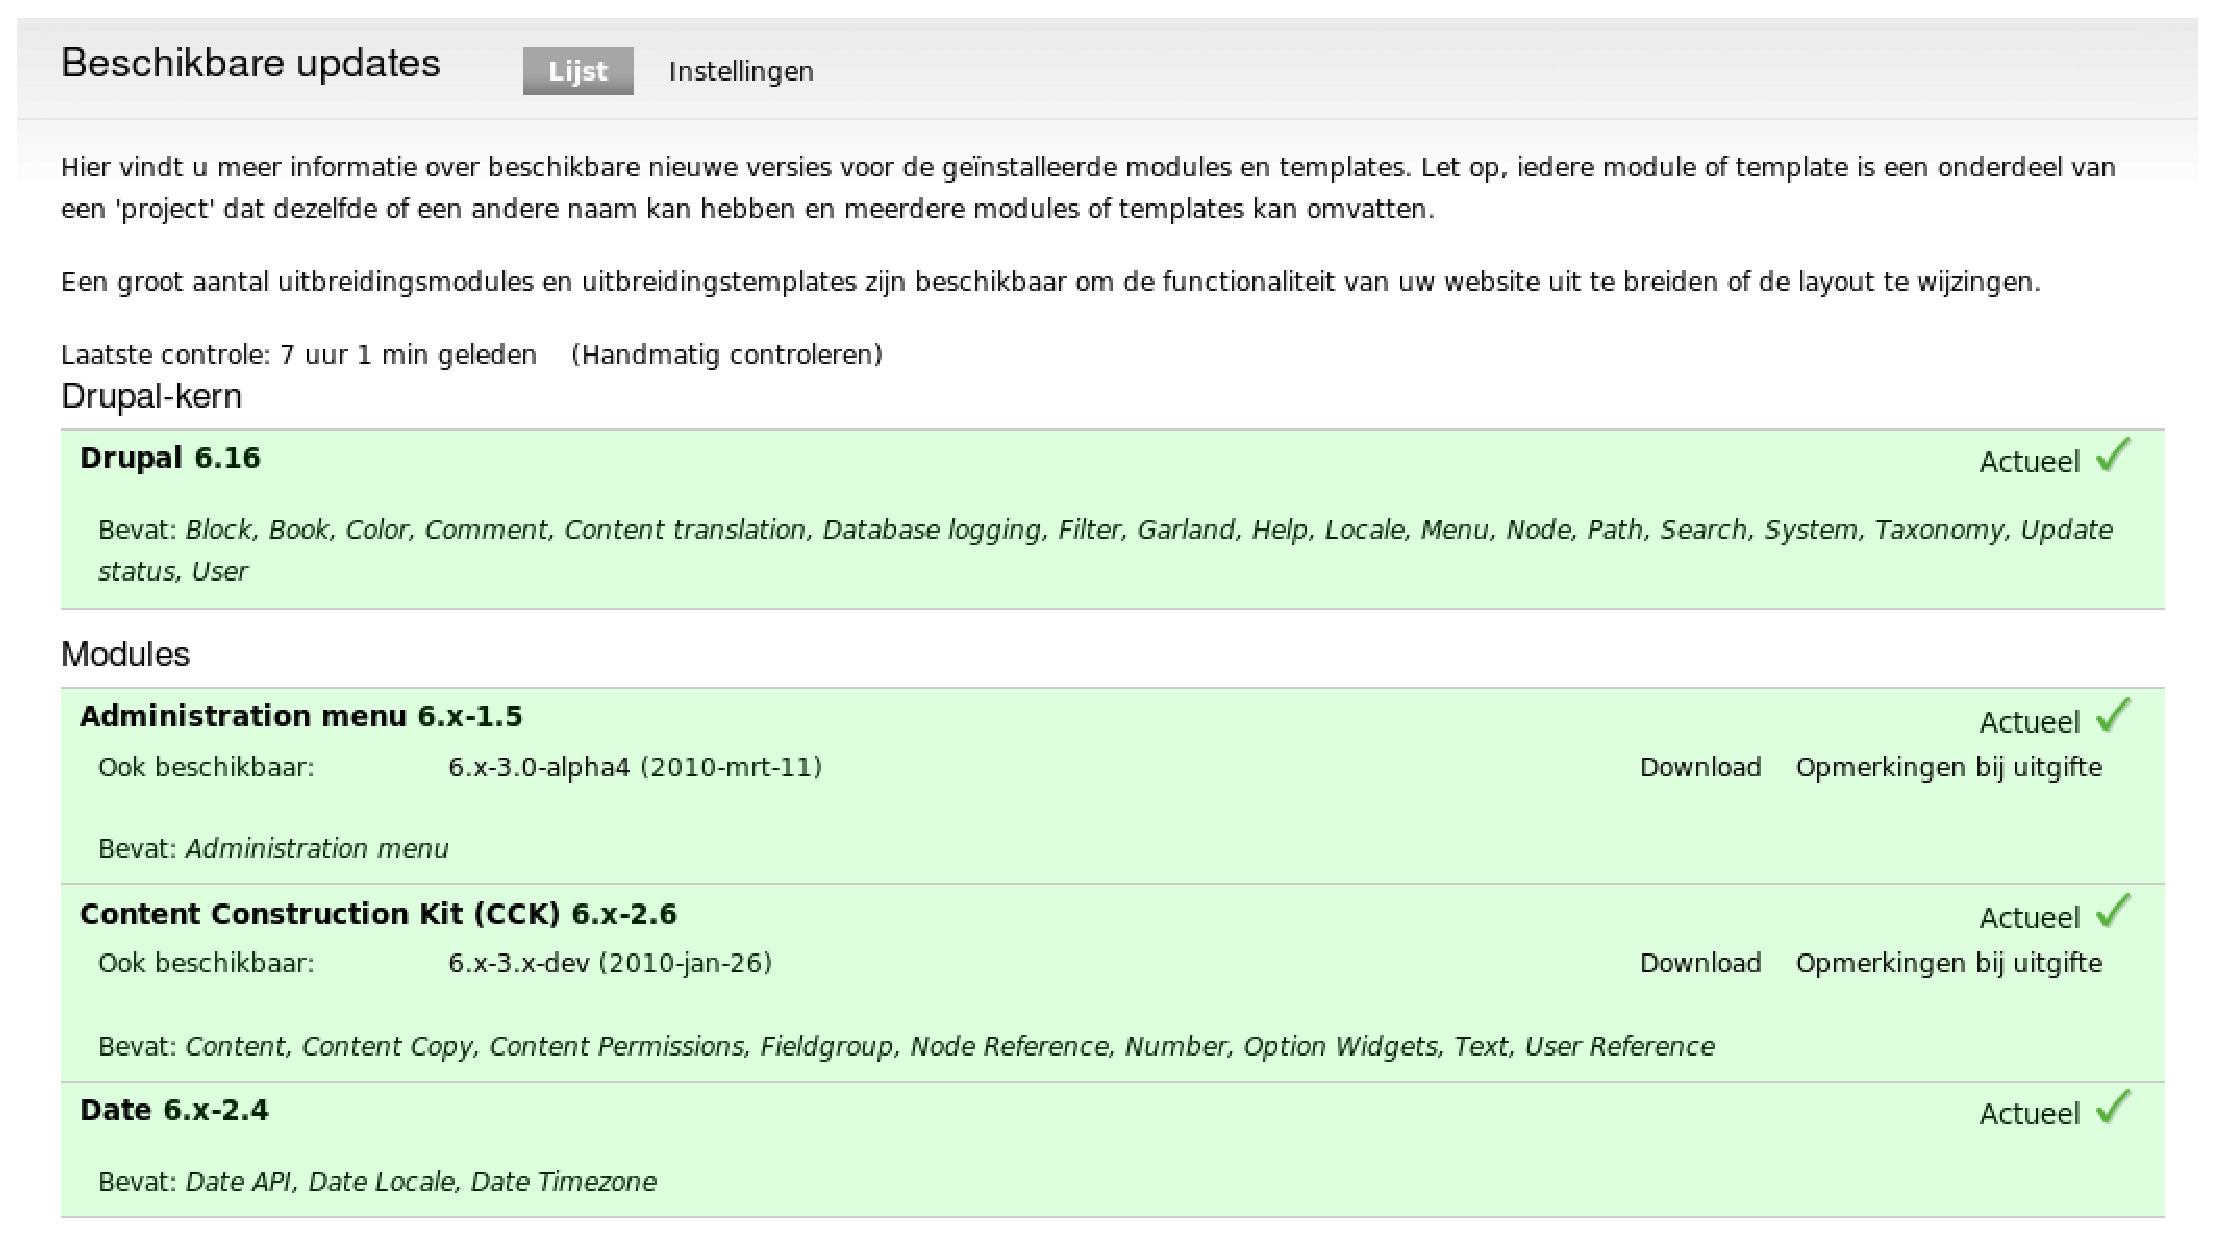
\includegraphics[scale=0.4,angle=0]{updates}
   \caption{updates.\label{white}}
 %  \small \\Drupal
 \end{figure}
 
\section{Status rapportage} \index{rapportage}
Weergave van de systeemstatus en eventueel gedetecteerde problemen.\\\\
Hier vindt u een kort overzicht van de parameters van uw site en eventuele
problemen met uw installatie. Het kan nuttig zijn deze informatie mee te geven bij het indienen van ondersteuningsvragen op de forums van drupal.org en in de project 'issue queues'.
 \begin{figure}[!h]
    \centering
   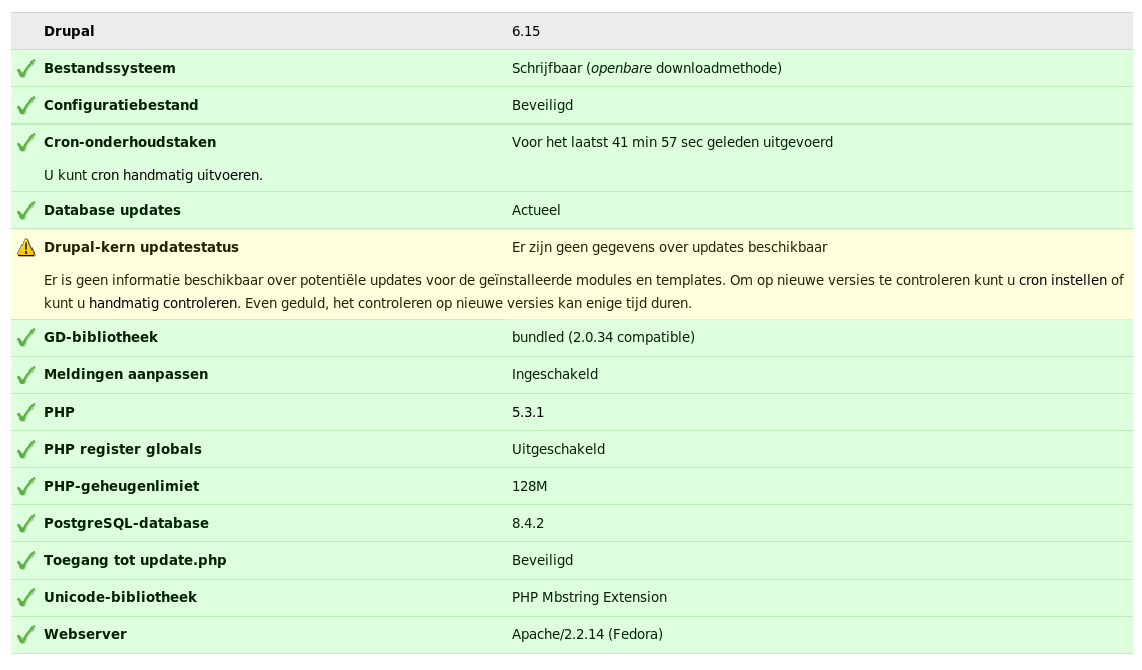
\includegraphics[scale=0.4,angle=0]{status_rapportage}
   \caption{Status rapportage.\label{white}}
 %  \small \\Drupal
 \end{figure}
